\section{Domäne}

Das nachfolgende Domänen-Modell zeigt alle nötigen Attribute für Umsetzung der Applikation. Es beinhaltet die angelieferten Daten von den Agenten (grün), die konfigurierbaren Daten, wie beispielsweise Benutzer, Rollen und Gruppenzugehörigkeiten (rot) und ausserdem die Informationen, welche für die Auftragsverwaltung benötigt werden (gelb).

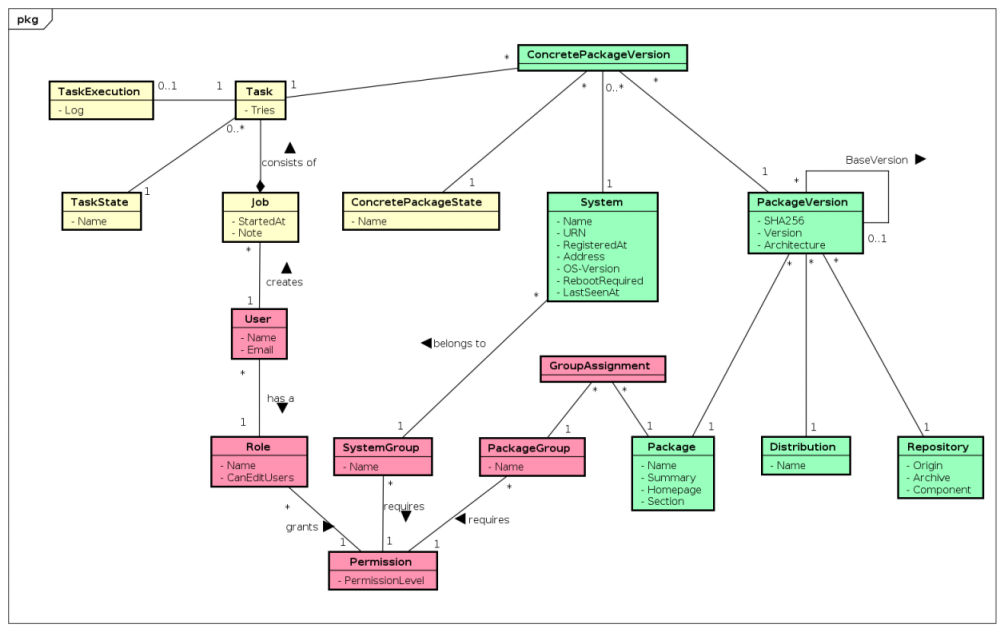
\includegraphics[width=\textwidth]{files/DomainModel_small}
\xxx[caption!]

\subsection*{Erläuterungen}

\subsubsection{System}

Ein System repräsentiert einen einzelnen Server, auf welchem die Updates verwaltet werden sollen. Relevante Daten über die Systeme werden erfasst respektive beim Registrieren durch den Agent mitgeteilt.

\subsubsection{Package}

Ein Package ist ein einzelnes Applikationspaket, welches vom Paketmanager (hier apt) verwaltet wird. Beispiele dafür sind vim, openssl oder sudo. Das Paket selbst ist unabhängig von Versionen oder Distributionen.

\subsubsection{PackageVersion}

Eine Paket-Version ist eine verfügbare Version eines bestimmten Paketes auf einem spezifischen Repository/einer Distribution.

\subsubsection{ConcretePackageVersion}

Eine Paket-Version kann mit einem System in Verbindung gebracht werden, zum Beispiel indem der Agent eine bestimmte Paket-Version als ausstehendes Update meldet. Diese Verbindung ist eine konkrete Paket-Version und zeigt, welchen Zustand diese Version auf diesem Paket hat: Installiert, veraltet, ausstehend, fehlgeschlagen oder in Auftrag gegeben.

\subsubsection{Distribution}

Eine Distribution, oft auch "Distro" genannt, ist ein Betriebssystem basierend auf dem Linux-Kernel. Beispiele: Debian, Suse oder Ubuntu. Diese werden wiederum in spezifische Distros unterteilt, etwa bei Ubuntu auf Ubuntu 12.04 precise, 14.04 trusty oder 16.04 xenial. 

\subsubsection{Job}

Ein Job wird dann erstellt, wenn ein Benutzer einen Auftrag erteilt. Pro betroffenem System enthält dieser Job einen Task, welcher dann an die Agenten geschickt wird.

\subsubsection{Task}

Ein Task enthält alle konkreten Aufträge für ein spezifisches System, welche von einem User in einem Durchgang erfasst wurden. Ein Task kann sich in den folgenden Zuständen befinden:

\begin{itemize}
    \item Erledigt 
    \item Fehlgeschlagen 
    \item Ausstehend
    \item In Bearbeitung
    \item Nicht zugestellt
\end{itemize}
